%% Photoionization cross sections in EXHALE: H I, He I, He II, He I 2^3 S
%% Comparison with Verner+1996 and the p-winds/Norcross tabulation.
%% Author: Kwang-Il Seon
\documentclass[english,a4paper]{my_memo}
\synctex=1
\usepackage{graphicx}
\usepackage{booktabs}
\usepackage{amsmath,amssymb}
\usepackage{listings}
\usepackage{xcolor}
\usepackage{babel}
\setlength{\emergencystretch}{3em}

\lstset{
  basicstyle=\ttfamily\footnotesize,
  keywordstyle=\color{blue}\bfseries,
  commentstyle=\color{gray},
  stringstyle=\color{olive},
  frame=single,
  breaklines=true,
  numbers=left,
  numberstyle=\tiny\color{gray},
  language=Python
}

\newcommand{\Mb}{\mathrm{Mb}}
\newcommand{\sig}{\sigma}

\begin{document}

\title{Photoionization Cross Sections in EXHALE:\\
H\,I, He\,I, He\,II, and the He\,I\,$2^3$S Triplet,\\
with Benchmarks against Verner+1996 and Norcross 1971}
\author{Kwang-Il Seon}
\date{2026-06-30}
\maketitle

\tableofcontents
\bigskip

%=============================================================================
\section{Overview}
%=============================================================================

EXHALE computes the photoionization rate of each species by integrating
its energy-dependent cross section $\sig(E)$ against the local stellar
spectrum on a fixed energy grid (the cross sections are pre-tabulated in
\texttt{set\_energy\_vectors.f90}). All cross-section routines live in
\texttt{src/modules/functions/cross\_sec.f90} (\texttt{module
Cross\_sections}) and return $\sig$ in units of
$1\,\Mb \equiv 10^{-18}\,\mathrm{cm}^2$, with photon energy $E$ in eV.

This memo (i) collects the four atomic cross sections relevant to the
He\,10830 / H$\alpha$ / Ly$\alpha$ diagnostics --- H\,I, He\,I, He\,II, and
the metastable He\,I\,$2^3$S triplet --- and (ii) benchmarks the two
\emph{fitted} helium cross sections against independent references:

\begin{itemize}
\item \textbf{He\,I ground state}: the EXHALE two-term ATES fit
  (\texttt{sigma\_HeI}) versus the Verner, Ferland, Korista \& Yakovlev
  (1996; hereafter VFKY96) single-shell analytic fit, over
  $24.6$--$500\,$eV.
\item \textbf{He\,I\,$2^3$S}: the EXHALE broken power-law fit
  (\texttt{sigma\_HeI23S}) versus the tabulation of Norcross (1971) data
  shipped with the \texttt{p-winds} code, over $4.77$--$60\,$eV.
\end{itemize}

All numbers and figures below are produced by the companion script
\texttt{docs/compare\_photoion\_cross\_sections.py}
(\S\ref{sec:script}), which ports the Fortran routines to Python verbatim
and writes vector-PDF figures into \texttt{docs/figures/}.

%=============================================================================
\section{The four cross sections}\label{sec:formulas}
%=============================================================================

\subsection{Hydrogenic atoms: H\,I and He\,II}

H\,I ($Z=1$) and He\,II ($Z=2$) use the analytic hydrogenic cross section
(\texttt{sigma(E,Z)}), with threshold $E_0 = 13.6\,Z^2\,$eV. For $E>E_0$,
\begin{equation}
  \sig(E) = \frac{6.3}{Z^2}\left(\frac{E_0}{E}\right)^{\!4}
            \frac{\exp\!\big[4 - 4\arctan(\epsilon)/\epsilon\big]}
                 {1 - \exp(-2\pi/\epsilon)}\;\Mb,
  \qquad \epsilon = \sqrt{E/E_0 - 1}\,,
\end{equation}
which is the exact non-relativistic result with the Gaunt-factor
correction; at threshold $\sig = 6.3/Z^2\,\Mb$ ($6.3\,\Mb$ for H\,I,
$1.575\,\Mb$ for He\,II).

\subsection{He\,I ground state (1$^1$S)}

By default the He\,I ground state (\texttt{sigma\_HeI}) uses the
Verner+1996 (VFKY96) single-shell fit --- the form of \S\ref{sec:vfky}
with the He\,I parameters of Table~\ref{tab:vfky}:
\begin{equation}
  \sig_{\rm He\,I}(E) = \sig_{\rm VFKY96}\!\big(E;\,
    E_{\rm th}{=}24.59,\,E_0{=}13.61,\,\sig_0{=}949.2,\,y_a{=}1.469,\,
    P{=}3.188,\,y_w{=}2.039,\,y_0{=}0.4434,\,y_1{=}2.136\big).
  \label{eq:heiverner}
\end{equation}
Setting \texttt{ATES\_photoionization\_rate: True} in \texttt{input.inp}
reverts to the legacy ATES two-term fit (valid above $E_{\rm th}=24.6\,$eV):
\begin{equation}
  \sig_{\rm He\,I}^{\rm ATES}(E) = \frac{0.6935}
       {(E/100)^{1.82} + (E/100)^{3.23}}\;\Mb .
  \label{eq:heiates}
\end{equation}
(The 2$^3$S metastable \emph{triplet} is a separate species,
Eq.~\ref{eq:he23s} below; Eqs.~\ref{eq:heiverner}--\ref{eq:heiates} are the
1$^1$S \emph{singlet} ground state only.)

\subsection{He\,I\,$2^3$S metastable (two VFKY96 forms $+$ bridge)}

The metastable triplet --- the lower level of He\,10830 ---
(\texttt{sigma\_HeI23S}) is built from \emph{two} Verner+1996 (VFKY96,
\S\ref{sec:vfky}) single-shell forms joined by a log-linear (power-law)
bridge, used piecewise. With $\ell\equiv\log_{10}(E/\mathrm{eV})$ and the
node energies $E_3{=}34.70$, $E_4{=}45.59\,$eV ($x_3{\equiv}\log_{10}E_3$,
$x_4{\equiv}\log_{10}E_4$):
\begin{equation}
\sig_{\rm He\,2^3S}(E) =
\begin{cases}
\sig_{\rm VFKY96}(E;\,\text{wing A}) & E\le E_3\quad(\text{threshold}\to\text{Cooper min})\\[2pt]
10^{\,m_b(\ell-x_3)+y_3^{b}} & E_3<E<E_4\quad(\text{power-law bridge})\\[2pt]
\sig_{\rm VFKY96}(E;\,\text{wing B}) & E\ge E_4\quad(\text{bump}\to\text{tail})
\end{cases}
\label{eq:he23s}
\end{equation}
Wing~A and wing~B use the parameters of Table~\ref{tab:he23svfky}
(\S\ref{sec:he23svfky}; each a $\sim$4\% fit to the resonance-averaged
cross section), and the bridge is the straight $\log$--$\log$ line joining
$y_3^{b}{=}\log_{10}\sig_{\rm VFKY96}(E_3;A)$ to
$y_4^{b}{=}\log_{10}\sig_{\rm VFKY96}(E_4;B)$ with
$m_b{=}(y_4^{b}-y_3^{b})/(x_4-x_3)$. Wing~A vanishes below the $4.78\,$eV
threshold (its $E_{\rm th}$), and wing~B supplies the smooth high-$E$ tail
($\sim E^{-7/2}$), so there is no hard cutoff. The construction is
continuous at both $E_3$ and $E_4$ and reproduces the former broken power
law to $\sim$4\% (deepest at the bump, $2.57$ vs $2.68\,\Mb$).

The \emph{former} five-segment broken power law (Norcross-1971 fit $+$
TOPbase-tail extension of \S\ref{sec:extend}), retained commented-out in
the code, was $\log_{10}\sig = -0.8134\,\ell{+}1.240$ ($4.78$--$7.49$),
$-1.772\,\ell{+}2.078$ ($7.49$--$34.70$), $9.098(\ell{-}x_3){-}0.6515$
($34.70$--$45.59$, the bump rise), $-2.660\,\ell{+}4.841$
($45.59$--$70$), and $-2.996\,\ell{+}5.462$ ($>70\,$eV, the TOPbase tail);
$\sig{=}0$ below $4.78\,$eV.

\subsection{Verner+1996 single-shell fit (VFKY96)}\label{sec:vfky}

This is the VFKY96 analytic fit, the form EXHALE adopts for metals, for
He\,II\footnote{via the hydrogenic routine} and --- now by default --- for
the He\,I ground state (\texttt{sigma\_VFKY96}); for $E\ge E_{\rm th}$,
\begin{align}
  x &= E/E_0 - y_0, \qquad z = \sqrt{x^2 + y_1^2}, \qquad
      Q = 5.5 - P/2, \\
  \sig(E) &= \sig_0\,\big[(x-1)^2 + y_w^2\big]\,
             z^{-Q}\,\big(1 + \sqrt{z/y_a}\big)^{-P}\;\Mb .
\end{align}
Verner+1996 Table~1 provides ground-shell parameters for \emph{all} ions
$Z=1$--$30$, including H\,I, He\,I and He\,II (Table~\ref{tab:vfky}); the
He\,I\,$2^3$S excited level is \emph{not} in that table, which is why a
separate Norcross-based fit is required for the triplet.

\begin{table}[h]
\centering
\caption{VFKY96 ground-shell parameters (Verner+1996 Table~1) used here.
$\sig_0$ in Mb.}
\label{tab:vfky}
\begin{tabular}{lrrrrrrr}
\toprule
ion & $E_{\rm th}$ & $E_0$ & $\sig_0$ & $y_a$ & $P$ & $y_w$ & $(y_0,y_1)$\\
\midrule
H\,I   & 13.60 & 0.4298 & $5.475\times10^4$ & 32.88 & 2.963 & 0.0   & $(0,0)$\\
He\,I  & 24.59 & 13.61  & 949.2             & 1.469 & 3.188 & 2.039 & $(0.4434,2.136)$\\
He\,II & 54.42 & 1.720  & $1.369\times10^4$ & 32.88 & 2.963 & 0.0   & $(0,0)$\\
\bottomrule
\end{tabular}
\end{table}

%=============================================================================
\section{Overview comparison}\label{sec:overview}
%=============================================================================

Figure~\ref{fig:overview} shows the four EXHALE-adopted cross sections on
a common log--log scale. The ordering of thresholds (He\,$2^3$S at
$4.78$, H\,I at $13.6$, He\,I at $24.6$, He\,II at $54.4\,$eV) and the
peak magnitudes ($\sim$$5$--$8\,\Mb$ near threshold for H\,I, He\,I and
He\,$2^3$S; $1.6\,\Mb$ for He\,II) are evident. The He\,$2^3$S curve
displays the characteristic minimum near $35\,$eV and the rise toward
$45\,$eV inherited from the Norcross data.

\begin{figure}[h]
\centering
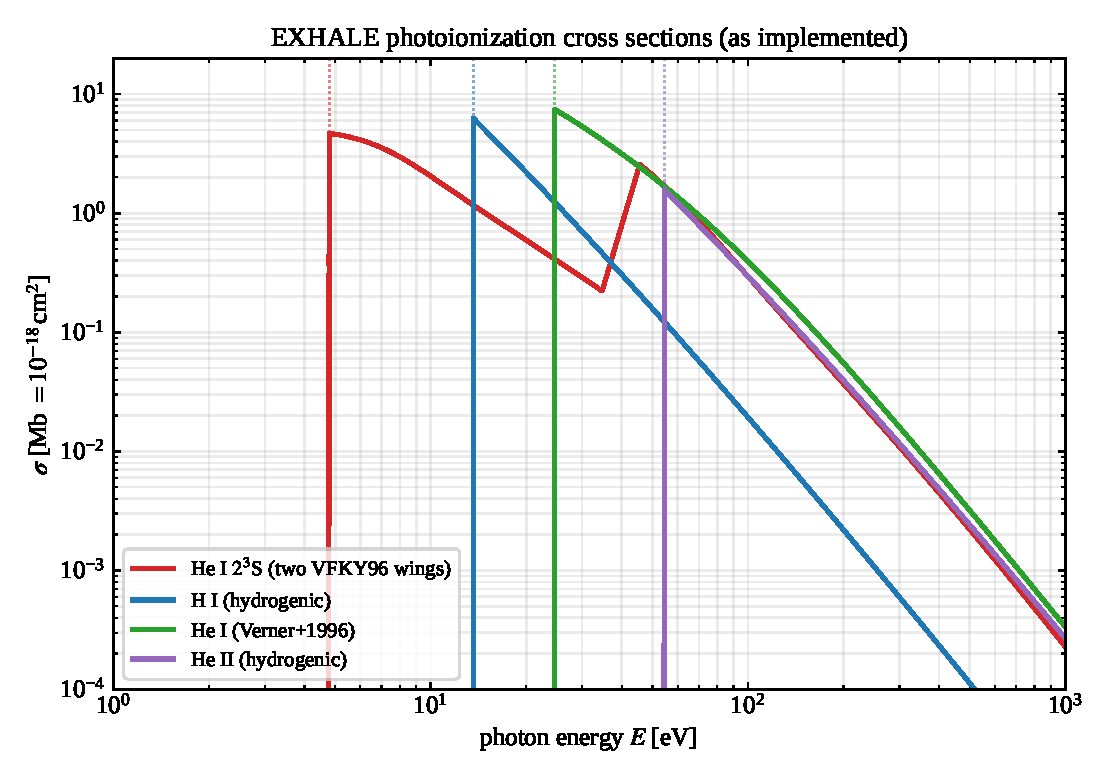
\includegraphics[width=0.82\textwidth]{figures/xsec_overview.pdf}
\caption{Photoionization cross sections adopted in EXHALE for H\,I, He\,I,
He\,II and the metastable He\,I\,$2^3$S triplet. Dotted vertical lines
mark the ionization thresholds.}
\label{fig:overview}
\end{figure}

%=============================================================================
\section{He\,I ground state: EXHALE two-term fit vs Verner+1996}
\label{sec:hei}
%=============================================================================

Figure~\ref{fig:hei} and Table~\ref{tab:hei} compare the EXHALE two-term
fit with the VFKY96 He\,I cross section over $24.6$--$500\,$eV. The two
agree to within $\sim$$14\%$ everywhere: the fits match within a few
percent at threshold and at high energy, with the two-term form running
$\sim$$12$--$14\%$ \emph{below} VFKY96 in the $50$--$100\,$eV range
(the band that dominates He photoionization in a typical XUV field). The
median ratio over the interval is $0.94$.

\begin{table}[h]
\centering
\caption{He\,I cross section (Mb): EXHALE two-term fit vs Verner+1996.}
\label{tab:hei}
\begin{tabular}{rrrr}
\toprule
$E$ [eV] & EXHALE & Verner & ratio\\
\midrule
24.6 & 7.821 & 7.430 & 1.053\\
30   & 5.244 & 5.361 & 0.978\\
50   & 1.779 & 2.022 & 0.880\\
100  & 0.347 & 0.394 & 0.880\\
200  & 0.054 & 0.055 & 0.973\\
300  & 0.0165& 0.0160& 1.028\\
500  & 0.0035& 0.0032& 1.089\\
\midrule
\multicolumn{4}{l}{ratio over $24.6$--$500\,$eV: min $0.861$, max $1.089$, median $0.939$}\\
\bottomrule
\end{tabular}
\end{table}

\begin{figure}[h]
\centering
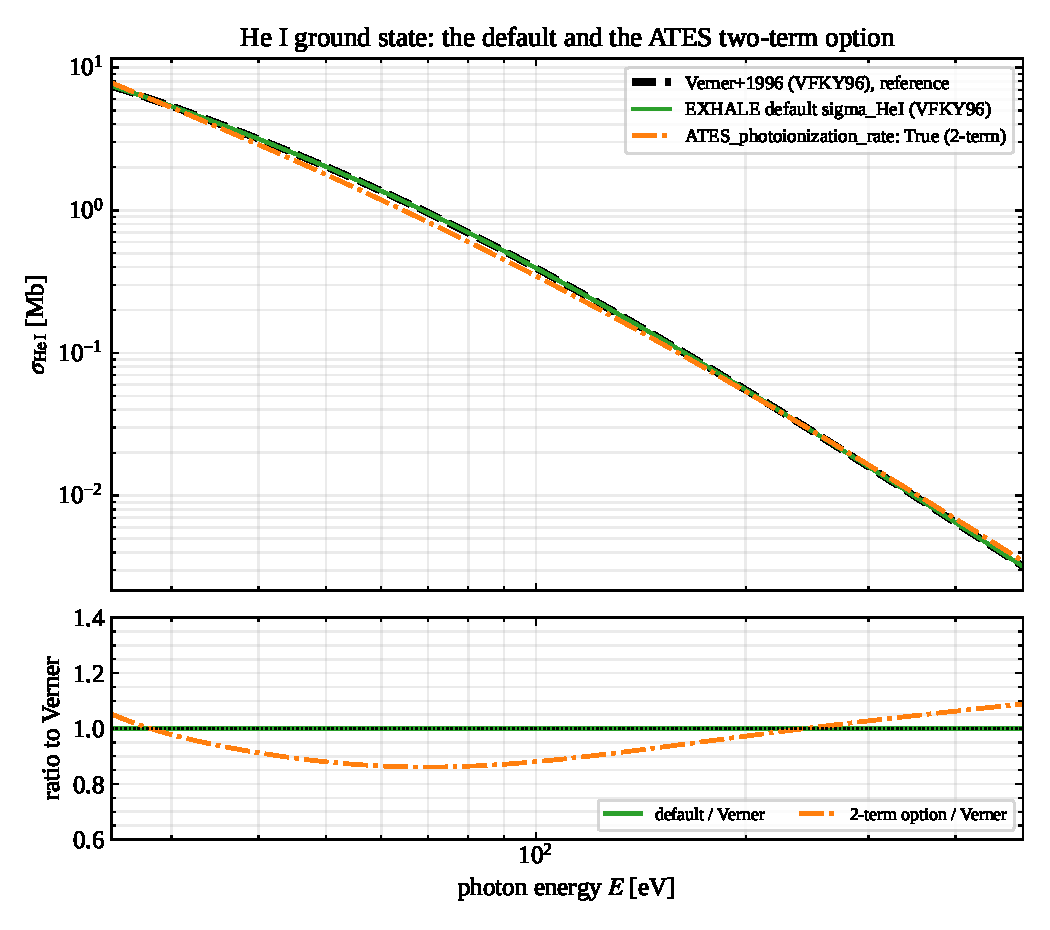
\includegraphics[width=0.72\textwidth]{figures/xsec_HeI_vs_Verner.pdf}
\caption{He\,I ground-state photoionization cross section: EXHALE two-term
fit (\texttt{sigma\_HeI}, green) vs the Verner+1996 single-shell fit
(black dashed). Bottom panel: ratio EXHALE/Verner.}
\label{fig:hei}
\end{figure}

Because both are accurate fits to the same underlying He\,I data, the
$\le 14\%$ difference is well within the photoionization-rate uncertainty
budget. Replacing \texttt{sigma\_HeI} with the VFKY96 He\,I parameters of
Table~\ref{tab:vfky} (a one-line wrapper around the existing
\texttt{sigma\_VFKY96}) would unify He\,I with the metal and He\,II
treatment and slightly improve the $50$--$100\,$eV band, but is not
required for the ionization balance.

%=============================================================================
\section{He\,I\,$2^3$S: EXHALE broken power law vs p-winds/Norcross}
\label{sec:he23s}
%=============================================================================

The \texttt{p-winds} code (dos Santos et al.\ 2022) ships the He\,$2^3$S
photoionization cross section as a 23-point table of Norcross (1971),
converting a differential oscillator strength $df/d\epsilon$ to a cross
section via $\sig[\mathrm{cm}^2] = 8.0670\times10^{-18}\,(df/d\epsilon)$.
Crucially, the EXHALE broken-power-law breakpoints coincide \emph{exactly}
with the Norcross wavelength nodes, confirming that \texttt{sigma\_HeI23S}
is a fit to this same data set.

Figure~\ref{fig:he23s} overlays the EXHALE curve, the tabulated Norcross
points, and their log--log interpolation; Table~\ref{tab:he23s} lists the
comparison. The agreement is excellent: the broken power law reproduces
the table to within $\sim$$10\%$ across $4.78$--$59\,$eV, with a median
ratio of $1.00$. The only localized deviation ($\sim$$15\%$) occurs right
at the Cooper minimum near $30\,$eV, where the cross section is smallest
and therefore least important for the rate.

\begin{table}[h]
\centering
\caption{He\,I\,$2^3$S cross section (Mb): EXHALE broken PL vs
p-winds/Norcross. (At threshold $4.78\,$eV the table interpolation is
undefined; EXHALE gives $4.867\,\Mb$, matching the Norcross threshold
value $8.0670\times0.605 = 4.881\,\Mb$.)}
\label{tab:he23s}
\begin{tabular}{rrrr}
\toprule
$E$ [eV] & EXHALE & p-winds & ratio\\
\midrule
6   & 4.046 & 4.092 & 0.989\\
8   & 3.006 & 3.110 & 0.966\\
12  & 1.465 & 1.463 & 1.002\\
20  & 0.593 & 0.546 & 1.085\\
30  & 0.289 & 0.277 & 1.042\\
45  & 2.382 & 2.442 & 0.975\\
55  & 1.517 & 1.516 & 1.001\\
59  & 1.226 & 1.251 & 0.980\\
\midrule
\multicolumn{4}{l}{ratio over $4.78$--$59\,$eV: min $0.853$, max $1.095$, median $1.000$}\\
\bottomrule
\end{tabular}
\end{table}

\begin{figure}[h]
\centering
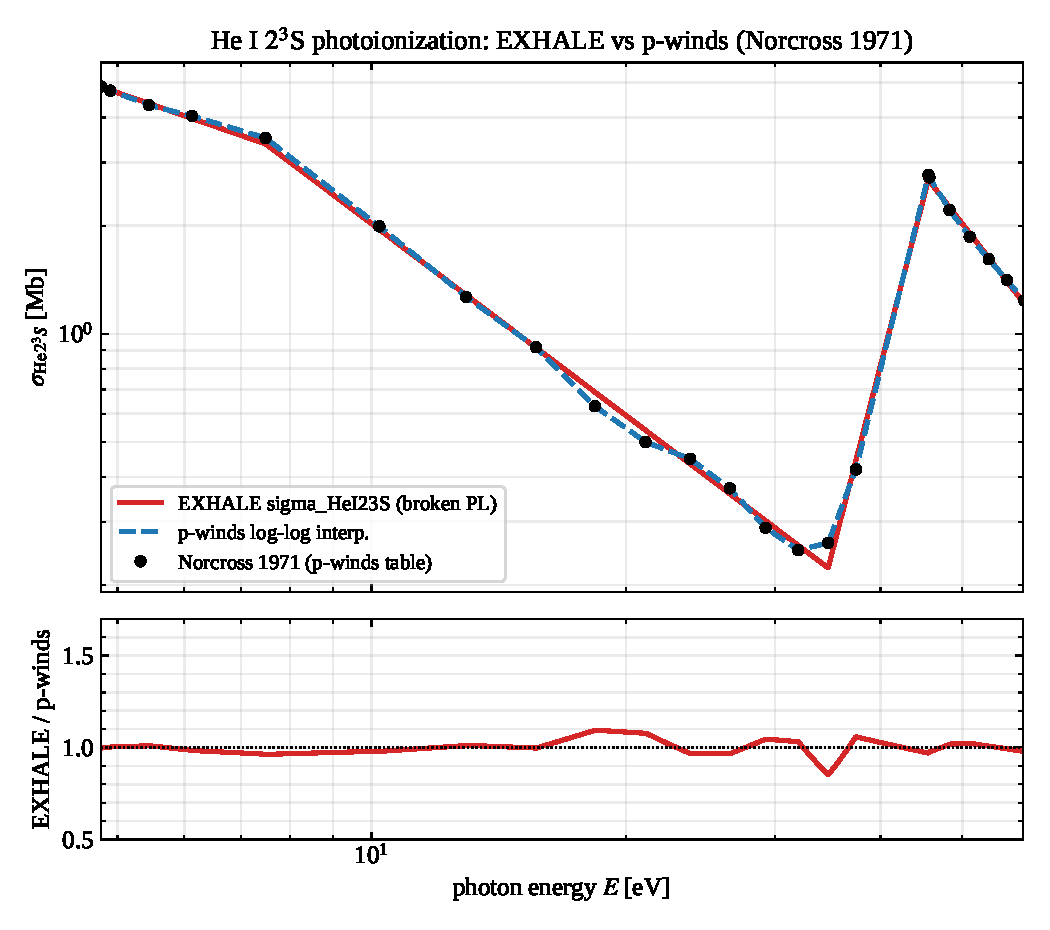
\includegraphics[width=0.72\textwidth]{figures/xsec_HeI23S_vs_pwinds.pdf}
\caption{He\,I\,$2^3$S photoionization cross section: EXHALE broken power
law (\texttt{sigma\_HeI23S}, red) vs the p-winds log--log interpolation
(blue dashed) of the Norcross (1971) table (black points). Bottom panel:
ratio EXHALE/p-winds.}
\label{fig:he23s}
\end{figure}

\subsection{Cross-check against TOPbase / Opacity Project}
\label{sec:topbase}

As an independent, fully \emph{ab initio} reference we extracted the
He\,I\,$2^3$S ($1s2s\,^3S$) photoionization cross section from the
\textbf{TOPbase} (Opacity Project) R-matrix database at the CDS server.
The relevant level is $\mathrm{NZ}=2$, $\mathrm{NE}=2$,
$\mathrm{iSLP}=300$ ($^3S$, even parity), $\mathrm{iLV}=1$; the table has
$922$ points with the photon energy in Rydberg and $\sig$ in Mb (level
energy $-0.35032\,$Ry, i.e.\ ionization threshold $4.766\,$eV). The query
URL and parsing are in the companion script (\S\ref{sec:script}); the raw
table is saved as \texttt{docs/data/topbase\_HeI\_2\_3S\_photo.dat}.

Two points must be kept in mind when comparing. (i) The TOPbase threshold
sits at the \emph{theoretical} energy ($4.63\,$eV for the first point),
$\sim$$0.14\,$eV below the experimental $4.77\,$eV; this is the usual OP
threshold offset. (ii) Above $\sim$$35\,$eV TOPbase resolves a dense
forest of \textbf{autoionizing resonances} (doubly-excited states
converging on the excited He\,II core), with peaks reaching
$\sig\simeq3200\,\Mb$. These are real but extremely narrow, and the
smooth Norcross/EXHALE fits represent only their resonance-averaged
background.

Figure~\ref{fig:topbase}(a) shows the full range with the resonance
structure; panel~(b) zooms into the smooth near-threshold region
($4.6$--$25\,$eV). In that smooth region the three independent
descriptions agree to within $\sim$$8\%$ (Table~\ref{tab:topbase}):
EXHALE/TOPbase has min $0.92$, max $1.07$, median $1.00$ over
$5$--$20\,$eV. This confirms that the EXHALE broken power law --- and the
Norcross data it is fit to --- reproduces the OP R-matrix background where
it matters for the He\,$2^3$S population.

Two caveats remain for completeness: (a) EXHALE sets
$\sig_{\rm He\,2^3S}=0$ above $59.2\,$eV, whereas TOPbase shows a smooth
$\sim$$E^{-3}$ tail continuing to several hundred eV (small in
magnitude, $\lesssim0.1\,\Mb$); (b) the broken-power-law ``bump'' near
$45\,$eV is a smooth stand-in for the resonance complex and should not be
read as a true cross section at any single energy there.

\begin{table}[h]
\centering
\caption{He\,I\,$2^3$S cross section (Mb) in the smooth near-threshold
region: EXHALE vs Norcross/p-winds vs TOPbase.}
\label{tab:topbase}
\begin{tabular}{rrrrrr}
\toprule
$E$ [eV] & EXHALE & p-winds & TOPbase & EX/TB & PW/TB\\
\midrule
5.0  & 4.693 & 4.671 & 5.081 & 0.924 & 0.919\\
6.0  & 4.046 & 4.092 & 4.231 & 0.956 & 0.967\\
8.0  & 3.006 & 3.110 & 2.866 & 1.049 & 1.085\\
10.0 & 2.024 & 2.069 & 2.025 & 1.000 & 1.022\\
12.0 & 1.465 & 1.463 & 1.488 & 0.985 & 0.983\\
16.0 & 0.880 & 0.872 & 0.877 & 1.004 & 0.994\\
20.0 & 0.593 & 0.546 & 0.574 & 1.033 & 0.952\\
\midrule
\multicolumn{6}{l}{EXHALE/TOPbase over $5$--$20\,$eV: min $0.924$, max $1.066$, median $0.999$}\\
\bottomrule
\end{tabular}
\end{table}

\begin{figure}[h]
\centering
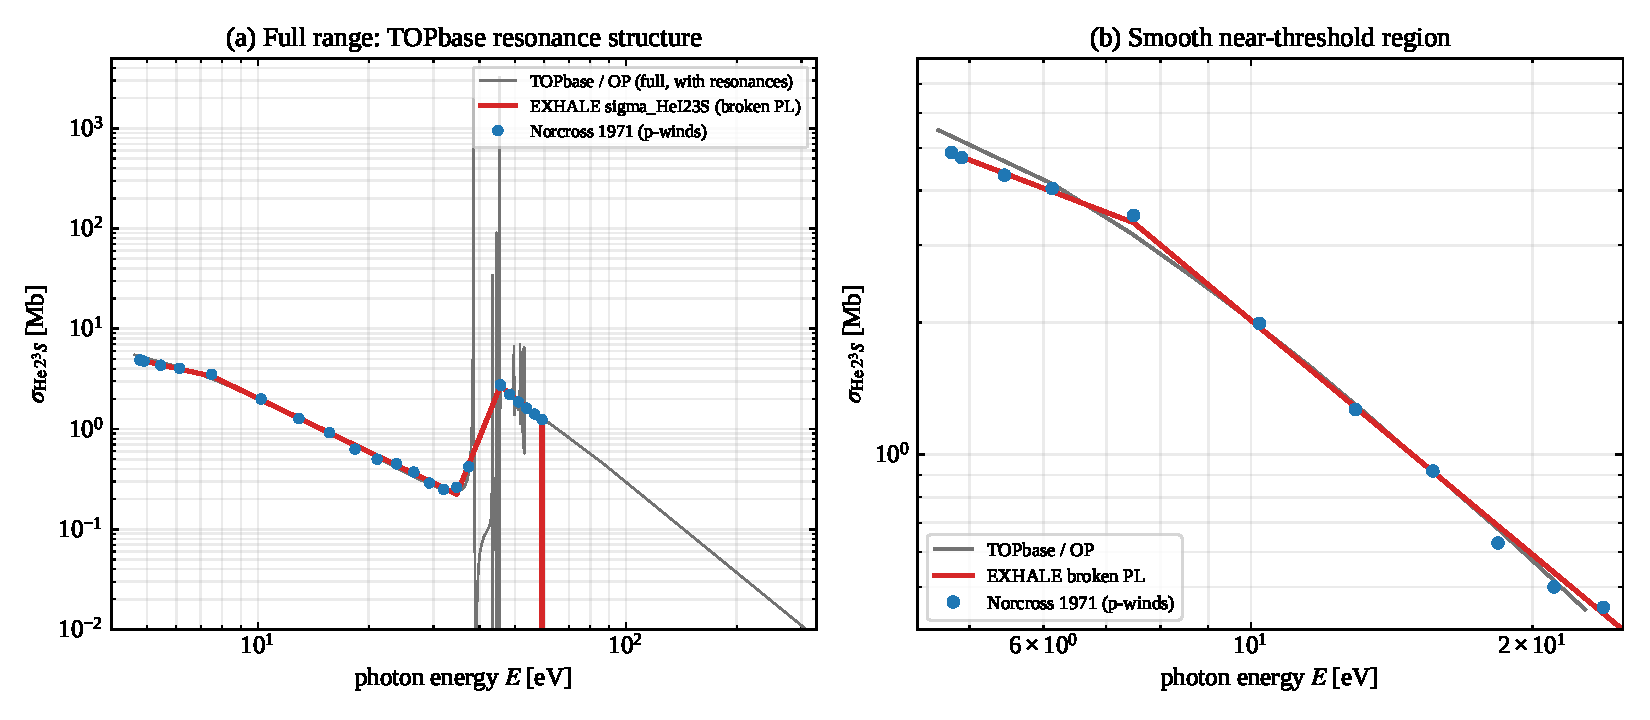
\includegraphics[width=0.98\textwidth]{figures/xsec_HeI23S_topbase.pdf}
\caption{He\,I\,$2^3$S photoionization: EXHALE broken power law (red),
Norcross/p-winds table (blue points), and TOPbase/OP (gray).
\textbf{(a)} Full range: TOPbase resolves autoionizing resonances above
$\sim$$35\,$eV (peaks to $\sim$$3200\,\Mb$) that the smooth fits average
over; EXHALE is truncated to zero above $59\,$eV. \textbf{(b)} Smooth
near-threshold region: the three agree to within $\sim$$8\%$.}
\label{fig:topbase}
\end{figure}

\subsection{Does the $>59\,$eV truncation matter for the rate?}
\label{sec:rateimpact}

The relevant quantity for the He\,$2^3$S population (and hence He\,10830)
is the \emph{photoionization rate},
$\Gamma_{2^3S} \propto \int \sig_{2^3S}(E)\,N(E)\,dE$, where
$N(E)=J_\nu/h\nu \propto J_{\rm inc}(E)/E$ is the photon-number flux.
In the EXHALE power-law SED, $J_{\rm inc}\propto E^{\rm PLind}$ over the
EUV band $[e_{\rm low},e_{\rm mid}]=[4.8,124]\,$eV (normalized to
$L_{\rm EUV}$) and the X-ray band $[124,1240]\,$eV (to $L_{\rm X}$), so
$N(E)\propto E^{\rm PLind-1}$. Because both $N(E)$ and $\sig_{2^3S}$ fall
steeply, the integrand peaks at the threshold; the rate is dominated by
the near-threshold UV ($\sim$$4.8$--$15\,$eV), where $\sig$ is largest
($1$--$5\,\Mb$) and photons are most numerous.

Table~\ref{tab:rateimpact} gives the relative increase of $\Gamma_{2^3S}$
when $\sig_{2^3S}$ is extended above $59.18\,$eV with the TOPbase tail
(integrated to $323\,$eV). The effect is only $0.1$--$1.2\%$ across
realistic spectral indices ($\mathrm{PLind}=-1$ to $-2$) and X-ray/EUV
ratios; for the EUV slopes typical of cool stars
($\mathrm{PLind}\simeq-1.3$ to $-1.6$) it is $0.3$--$0.6\%$. This is far
below the $\sim$$10\%$ uncertainty of the cross-section fit itself
(\S\ref{sec:he23s}) and of the composition/SED. The $35$--$59\,$eV
resonance ``bump'' likewise carries only $\sim$$2\%$ of the current rate.

Moreover, these are \emph{upper bounds}: the power-law SED extrapolates
the EUV slope down to $4.8\,$eV, whereas a real star has a much larger
photospheric near-UV flux ($4.8$--$13.6\,$eV); with a realistic SED the
near-threshold region dominates even more and the $>59\,$eV contribution
shrinks further. (Heating is also unaffected: the $2^3S$ number density
is negligible compared with the H/He ground states, so its
photoionization deposits negligible energy regardless of the high-energy
tail.) We therefore retain the $59\,$eV cutoff; extending it is a
cosmetic, sub-percent refinement.

\begin{table}[h]
\centering
\caption{Relative increase (\%) of the He\,$2^3$S photoionization rate
when $\sig_{2^3S}$ is extended above $59\,$eV with the TOPbase tail, for
an EXHALE power-law SED of index PLind and X-ray/EUV luminosity ratio
$L_{\rm X}/L_{\rm EUV}$.}
\label{tab:rateimpact}
\begin{tabular}{rrrr}
\toprule
PLind & $L_{\rm X}/L_{\rm EUV}=0.1$ & $0.3$ & $1.0$\\
\midrule
$-1.0$ & 1.13\% & 1.15\% & 1.21\%\\
$-1.3$ & 0.57\% & 0.59\% & 0.65\%\\
$-1.6$ & 0.29\% & 0.30\% & 0.36\%\\
$-2.0$ & 0.12\% & 0.13\% & 0.19\%\\
\bottomrule
\end{tabular}
\end{table}

\subsection{Impact of the autoionizing resonances}
\label{sec:resonance}

Between $\sim$$40$ and $55\,$eV, TOPbase shows a dense forest of
autoionizing resonances (doubly-excited states converging on the
He\,II\,$n=2$ threshold at $65.4\,$eV), with peaks reaching
$\sig\simeq3223\,\Mb$, whereas the EXHALE broken power law represents this
region by a smooth bump peaking at only $\sim$$2.4\,\Mb$
(Fig.~\ref{fig:topbase}a). It is tempting to ask whether the resonances,
being so tall, substantially raise the He\,$2^3$S photoionization rate.

\textbf{They do not} --- but the analysis requires care, because
\emph{the raw TOPbase table must not be integrated directly}. Integrating
both cross sections on the \emph{same} native TOPbase energy grid (so the
quadrature is identical) gives the total-rate ratio TOPbase/EXHALE in
Table~\ref{tab:resonance}. With no clipping the resonances appear to raise
the rate by $\sim$$13\%$ (at $\mathrm{PLind}=-1.3$); but this increase is
produced almost entirely by the $2$--$4$ tallest grid points. The
narrowest resonances ($\Delta E\sim0.01\,$eV) are sampled by only one or
two points, so the trapezoidal rule assigns them a triangular area fixed
by the arbitrary mesh spacing rather than by the physical Lorentzian
width. Clipping $\sig$ at $\gtrsim100\,\Mb$ removes just these few
unresolved spikes and the ratio collapses to $0.99$--$1.02$: \textbf{the
robust net effect of the resonances on the rate is only $\sim$$1$--$2\%$.}

\begin{table}[h]
\centering
\caption{Convergence/spike test of the resonance contribution. Total
He\,$2^3$S rate ratio TOPbase/EXHALE ($\mathrm{PLind}=-1.3$), both
integrated on the same native grid, as the TOPbase cross section is
clipped at an upper value; ``pts$>$cap'' counts the grid points removed.}
\label{tab:resonance}
\begin{tabular}{rrr}
\toprule
$\sig$ clip [Mb] & TOPbase/EXHALE & pts $>$ cap\\
\midrule
none (raw) & 1.134 & 0\\
500 & 1.024 & 2\\
200 & 1.001 & 2\\
100 & 0.993 & 4\\
50  & 0.989 & 7\\
\bottomrule
\end{tabular}
\end{table}

Physically this is expected: although individual resonances are very
tall, they are extremely narrow and therefore intercept little photon
flux. The resonance-\emph{averaged} cross section
$\langle\sig\rangle = \sig_{\rm bg} + \sum_i (\text{resonance area})_i/\Delta E$
sits only modestly above the smooth background, which the few-Mb
Norcross/EXHALE values already approximate. The net resonance effect
($\sim$$1$--$2\%$) is comparable to the $>59\,$eV tail
(\S\ref{sec:rateimpact}) and well below the $\sim$$10\%$ fit and
composition/SED uncertainties, so it does not change the He\,10830
conclusions.

\textbf{Practical caveat:} for percent-level work one must use a properly
resonance-averaged Opacity-Project cross section (e.g.\ the
resonance-averaged tabulations in the spirit of Bautista et al.); the raw
$922$-point TOPbase table should never be fed into a broadband rate
integral, as the quadrature artifact in Table~\ref{tab:resonance}
illustrates.

\subsection{A smooth high-energy extension ($E>59\,$eV)}
\label{sec:tail}

Although the $>59\,$eV truncation is dynamically harmless
(\S\ref{sec:rateimpact}), a smooth analytic extension is trivial to
provide and removes the (cosmetic) hard cutoff. Above the He\,II\,$n=2$
resonance limit ($E\gtrsim66\,$eV) the TOPbase cross section is smooth and
monotonic, and a single power law fits the resonance-free background to
$\sim$$5\%$ over $60$--$320\,$eV (Fig.~\ref{fig:tail}):
\begin{equation}
\boxed{\;\sig_{\rm He\,2^3S}(E) \simeq 0.294\,
   \left(\frac{E}{100\,\text{eV}}\right)^{-2.99}\,\Mb
   \;=\; 10^{5.45}\,E^{-2.99}\ \Mb \quad (E>59\,\text{eV}),\;}
\end{equation}
with $E$ in eV. The index $-2.99$ is close to the asymptotic hydrogenic
$s$-shell value ($-7/2$ is approached only at much higher $E$), and the
fit residuals are $\le0.023\,$dex. This is the resonance-\emph{free}
background by construction: it is fit only to points above the $n=2$
resonance limit and deliberately ignores the $40$--$55\,$eV resonance
forest (\S\ref{sec:resonance}).

To splice it into \texttt{sigma\_HeI23S}, replace the ``zero above $x_5$''
branch with one more log-linear segment of slope $-2.99$. Two variants:
(i) \emph{data-matched} --- use the boxed normalization, which reproduces
TOPbase to $5\%$ but sits $\sim$$16\%$ above the broken-PL endpoint at the
$59.2\,$eV junction (a step at $\sig\sim1.4\,\Mb$, irrelevant to the rate);
(ii) \emph{continuity-matched} --- anchor at the broken-PL value
$\sig(59.2)=1.21\,\Mb$, i.e.\ $\sig=1.21\,(E/59.2)^{-2.99}\,\Mb$, which is
continuous but runs $\sim$$15\%$ below TOPbase. Either is adequate; given
the $<1\%$ rate impact, the continuity-matched form is the tidier drop-in.

\begin{figure}[h]
\centering
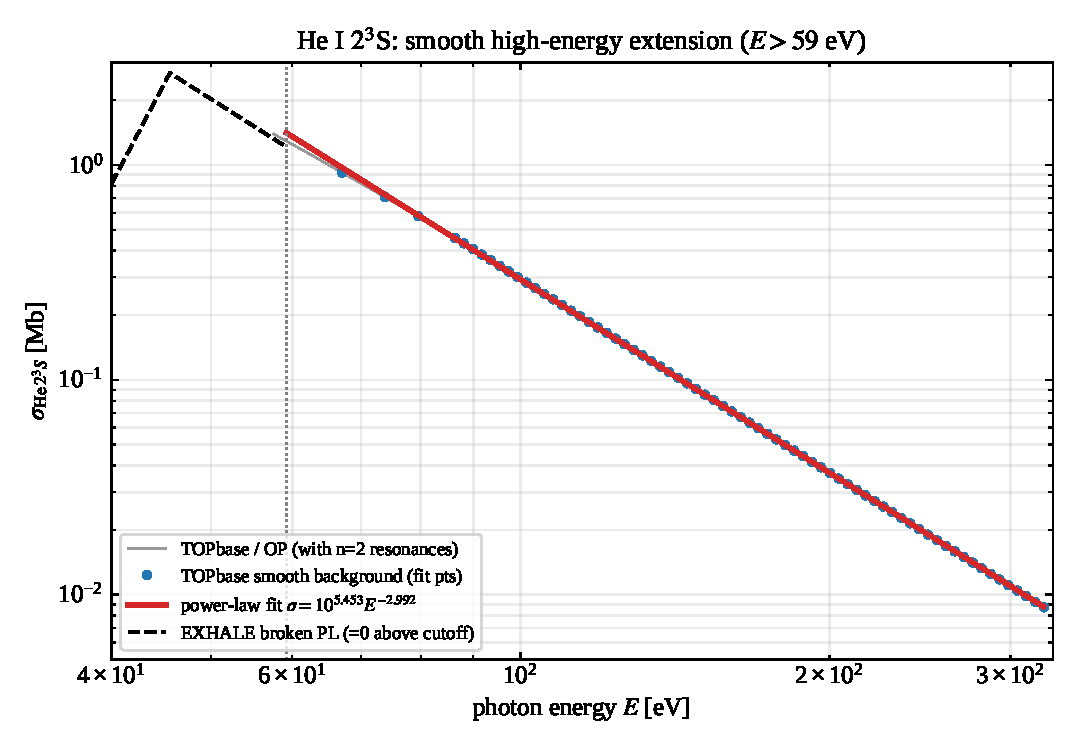
\includegraphics[width=0.72\textwidth]{figures/xsec_HeI23S_tail.pdf}
\caption{Smooth high-energy extension of $\sig_{\rm He\,2^3S}$. The
power-law fit (red) to the resonance-free TOPbase background (blue points,
$E\ge66\,$eV) follows $\sig\propto E^{-2.99}$ to $\sim$5\% up to
$320\,$eV. The current EXHALE broken power law (black dashed) rises to a
resonance-averaged bump near $45\,$eV and is cut to zero above
$59.2\,$eV (dotted line).}
\label{fig:tail}
\end{figure}

\subsection{A unified full-range representation from TOPbase}
\label{sec:unified}

The power-law tail of \S\ref{sec:tail} only patches the high-energy end.
A cleaner option is a single representation that follows the TOPbase
\emph{resonance-averaged} background over the whole range, $4.77$--$320\,$eV,
with no ad-hoc junction. Because the cross section has a deep Cooper
minimum near $30\,$eV, a resonance-averaged enhancement (the He\,II\,$n=2$
channel) peaking near $50\,$eV, and an $E^{-3}$ tail, no single compact
analytic form captures it. Instead we tabulate a short
$(E,\sig)$ node table and interpolate it \textbf{log--log with a monotone
cubic (PCHIP)} --- exactly the scheme EXHALE already uses for the metal
cooling fits, so it is a drop-in. Below $30\,$eV and above $66\,$eV the
nodes are the clean TOPbase background; in $30$--$66\,$eV they are the
\emph{resonance-averaged} (spike-capped) values, i.e.\ the sharp
resonances are deliberately averaged over rather than followed.

\begin{table}[h]
\centering
\caption{Node table for the unified He\,$2^3$S photoionization cross
section (log--log PCHIP interpolation; $\sig=0$ outside the range).}
\label{tab:unified}
\small
\begin{tabular}{lrrrrrrrrrrrrrrr}
\toprule
$E$ [eV]   & 4.77 & 6 & 8 & 10 & 13.6 & 20 & 30 & 40 & 52 & 63 & 80 & 100 & 150 & 200 & 300\\
$\sig$ [Mb] & 4.88 & 4.09 & 3.11 & 2.07 & 1.16 & 0.55 & 0.273 & 0.50 & 1.9 & 1.14 & 0.577 & 0.294 & 0.085 & 0.037 & 0.0111\\
\bottomrule
\end{tabular}
\end{table}

This representation (Fig.~\ref{fig:unified}) reproduces the TOPbase smooth
background to within $\sim$$10\%$ across the full range (the residual at
the very threshold is the $\sim$$0.14\,$eV theoretical-threshold offset,
\S\ref{sec:topbase}), is $C^1$-continuous by construction, and avoids the
hard cutoff. Crucially, the He\,$2^3$S photoionization \emph{rate} it
produces differs from the current broken power law by only $+1.7\%$
(PLind $=-1.3$; consistent with \S\ref{sec:rateimpact} and
\S\ref{sec:resonance}), confirming that the upgrade is a fidelity/
tidiness improvement rather than a change that moves the He\,10830
prediction. The $30$--$66\,$eV nodes carry the largest uncertainty
($\sim$$30\%$, from the resonance averaging) but the least weight.

\begin{figure}[h]
\centering
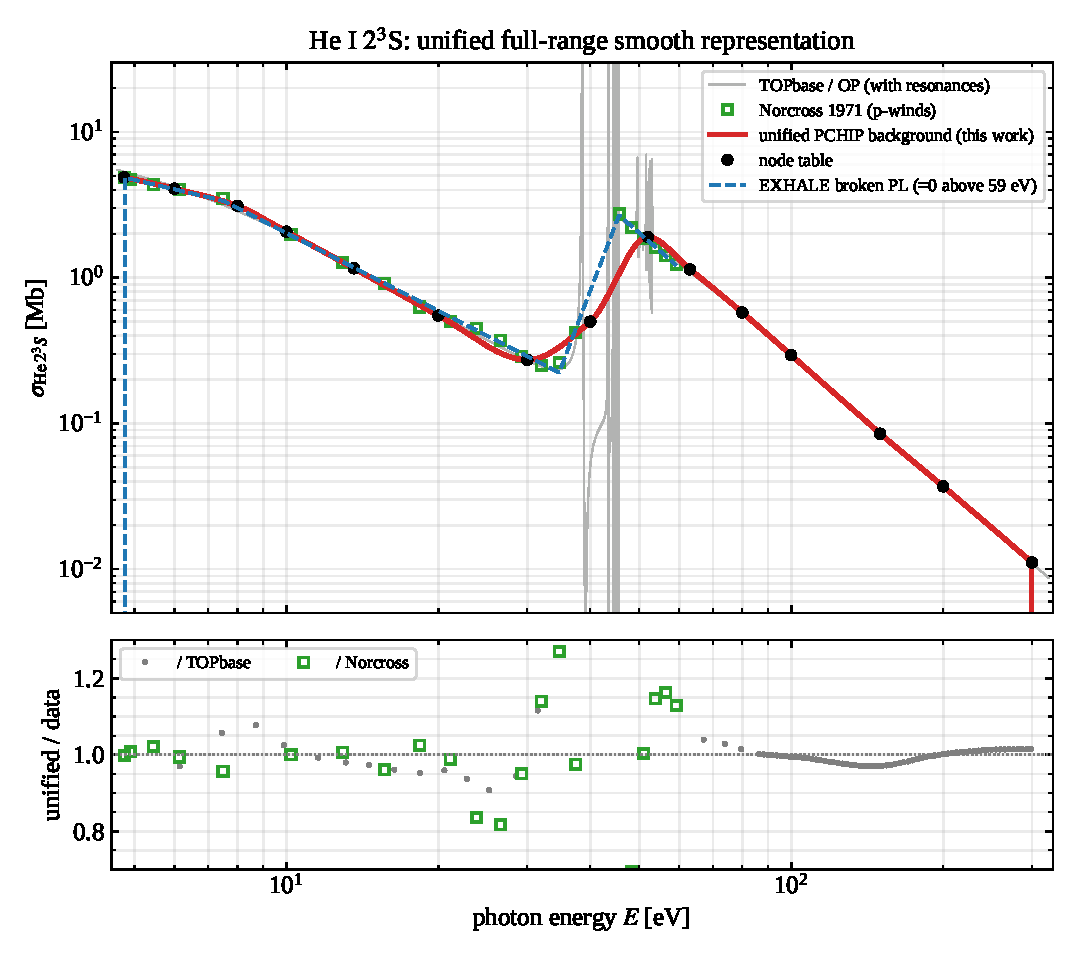
\includegraphics[width=0.82\textwidth]{figures/xsec_HeI23S_unified.pdf}
\caption{Unified full-range representation (red) of $\sig_{\rm He\,2^3S}$:
log--log PCHIP through the node table (black points; Table~\ref{tab:unified})
following the TOPbase resonance-averaged background (gray, with
resonances). The Norcross (1971) / p-winds table (green squares) and the
current EXHALE broken power law (blue dashed; cut to zero above $59\,$eV)
are overplotted. Bottom: ratio of the unified fit to the TOPbase
smooth-background points (gray) and to the Norcross points (green); both
within $\sim$$\pm15\%$, with the larger Norcross scatter at $40$--$55\,$eV
reflecting its coarse sampling of the resonance region.}
\label{fig:unified}
\end{figure}

\textbf{Recommendation.} For a clean, well-connected cross section over
all energies, adopt the Table~\ref{tab:unified} node set with log--log
PCHIP in \texttt{sigma\_HeI23S}. It is faithful to the OP R-matrix
background, smooth everywhere, and changes the rate by $<2\%$. If instead
only the cutoff is to be removed with minimal code change, the
continuity-matched power-law tail of \S\ref{sec:tail} suffices --- or,
better, the minimal-change extension of \S\ref{sec:extend} below.

\subsection{Recommended minimal-change extension}\label{sec:extend}

The tidiest upgrade keeps essentially all of the existing broken power law
and changes only its \emph{last} segment. The procedure is:
\begin{enumerate}
\item Keep the broken power law unchanged up to the resonance-averaged
  bump peak at $x_4$ ($45.6\,$eV; $\sig=2.68\,\Mb$) --- i.e.\ segments
  $a_1$, $a_2$ and the rising segment are untouched.
\item Fit the smooth TOPbase background above $E_J=70\,$eV with a power
  law:
  \begin{equation}
    \sig_{\rm tail}(E) = 10^{5.462}\,E^{-2.996}\;\Mb \qquad (E>70\,\text{eV}),
  \end{equation}
  ($\sig_{\rm TOPbase}(70\,\text{eV})=0.858\,\Mb$; fit residuals $\le3\%$).
\item Re-aim the last power-law segment so it runs from the bump peak at
  $x_4$ to exactly $\sig_{\rm tail}(70\,\text{eV})$ at $70\,$eV: its slope
  changes only slightly, from $-3.039$ to $\mathbf{-2.658}$
  (intercept $c_3=4.838$ in $\log_{10}\sig = a_3'\log_{10}E + c_3$).
  Above $70\,$eV use $\sig_{\rm tail}$; drop the old $59\,$eV cutoff.
\end{enumerate}
By construction the result is continuous at \emph{both} joins --- at
$45.6\,$eV (with the kept rising segment) and at $70\,$eV (with the
TOPbase tail) --- so there is no step and no kink beyond the tiny
$0.38$-in-slope change. It reproduces the TOPbase background to
$\sim$$3\%$ above $70\,$eV and tracks Norcross/p-winds throughout
(Fig.~\ref{fig:ext}), while changing the He\,$2^3$S photoionization rate
by only $+0.65\%$ (PLind $=-1.3$) --- the smallest of all the options.
This is the recommended drop-in: it is a one-line slope change plus a new
tail branch in \texttt{sigma\_HeI23S}, retains the validated
threshold-to-bump shape exactly, and removes the unphysical cutoff.

\begin{figure}[h]
\centering
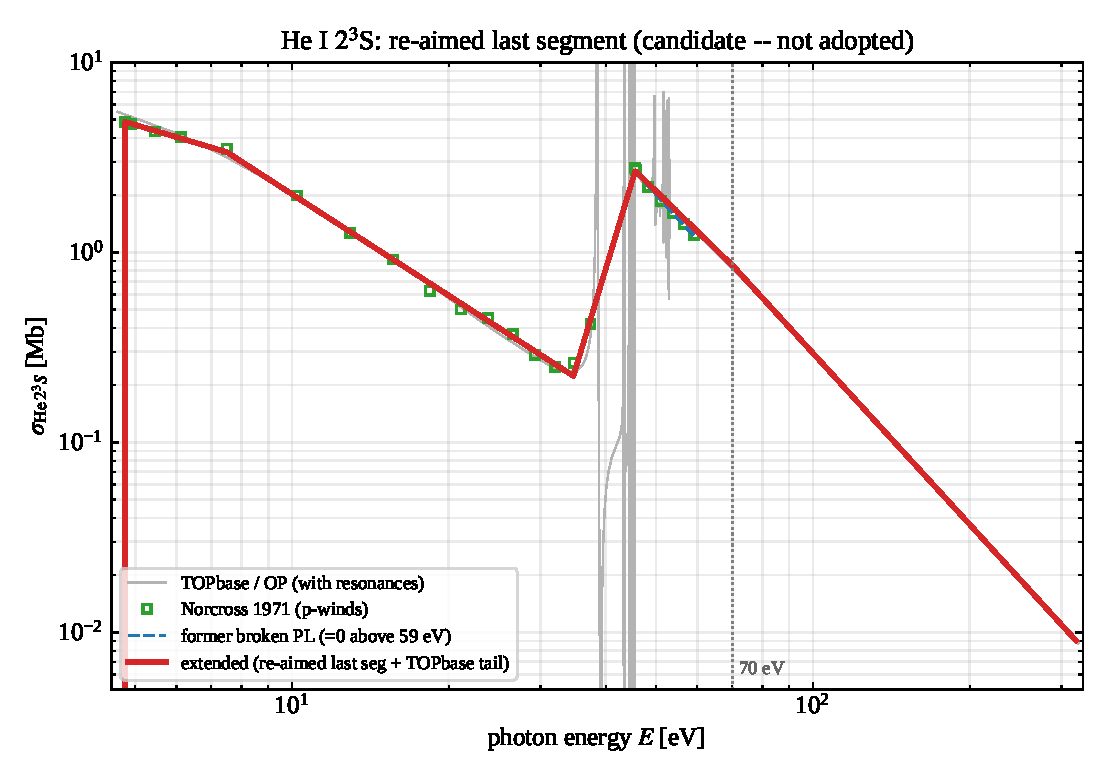
\includegraphics[width=0.78\textwidth]{figures/xsec_HeI23S_ext.pdf}
\caption{Recommended minimal-change extension (red): the original broken
power law up to the $45.6\,$eV bump, a re-aimed last segment (slope
$-3.039\!\to\!-2.658$) reaching the TOPbase fit at $70\,$eV (dotted line),
and the TOPbase power-law tail above. Norcross/p-winds (green) and TOPbase
(gray) are overplotted; the original broken power law (blue dashed) cuts
to zero at $59\,$eV. The curve is continuous at both joins.}
\label{fig:ext}
\end{figure}

\subsection{He\,$2^3$S as two VFKY96 (Verner) forms}\label{sec:he23svfky}

It is natural to ask whether the He\,$2^3$S cross section could use the same
VFKY96 fits (\S\ref{sec:vfky}) EXHALE already applies to He\,I and the
metals, instead of the bespoke broken power law. Fitting a \emph{single}
VFKY96 term to each smooth part of the curve works very well
(Fig.~\ref{fig:he23svfky}, Table~\ref{tab:he23svfky}): segments 1--2
(threshold $\to$ Cooper minimum, $4.85$--$34.7\,$eV) and segments 4--5
(resonance-averaged bump $\to$ tail, $45.7$--$320\,$eV) are \emph{each}
reproduced to $\sim$$4\%$. This is physically sensible --- the two terms are
the $2s$-shell channel and the (resonance-averaged) He\,II\,$n=2$ channel.

The one region the two wings do not cover is the \emph{transition}
($34.7$--$45.6\,$eV, shaded in Fig.~\ref{fig:he23svfky}), where the cross
section climbs from the Cooper minimum to the bump. This is bridged by a
short log-linear (power-law) segment joining wing~A at $E_3=34.70\,$eV to
wing~B at $E_4=45.59\,$eV. \textbf{This two-VFKY96-plus-bridge form is now
the EXHALE implementation} of \texttt{sigma\_HeI23S} (Eq.~\ref{eq:he23s});
it reproduces the former broken power law to $\sim$4\% (deepest at the
bump, $2.57$ vs $2.68\,\Mb$), is continuous at $E_3$ and $E_4$, and reuses
the same \texttt{sigma\_VFKY96} routine as He\,I and the metals. The former
broken power law is retained, commented out, in the code.

\begin{table}[h]
\centering
\caption{Single-VFKY96 fits to the two smooth parts of He\,$2^3$S (form of
\S\ref{sec:vfky}; $\sig_0$ in Mb, energies in eV). Each reproduces its
region to $\sim$4\%.}
\label{tab:he23svfky}
\begin{tabular}{lrrrrrrrr}
\toprule
region & $E_{\rm th}$ & $E_0$ & $\sig_0$ & $y_a$ & $P$ & $y_w$ & $y_0$ & $y_1$\\
\midrule
seg 1--2 ($4.85$--$34.7$)  & 4.78  & 2.645 & 20.8  & $1.0{\times}10^{12}$ & 3.42 & 2.681 & 1.956 & 2.603\\
seg 4--5 ($45.7$--$320$)   & 45.59 & 49.68 & 1052  & 0.0439 & 2.941 & 1.717 & $5.5{\times}10^{-5}$ & 1.118\\
\bottomrule
\end{tabular}
\end{table}

\begin{figure}[h]
\centering
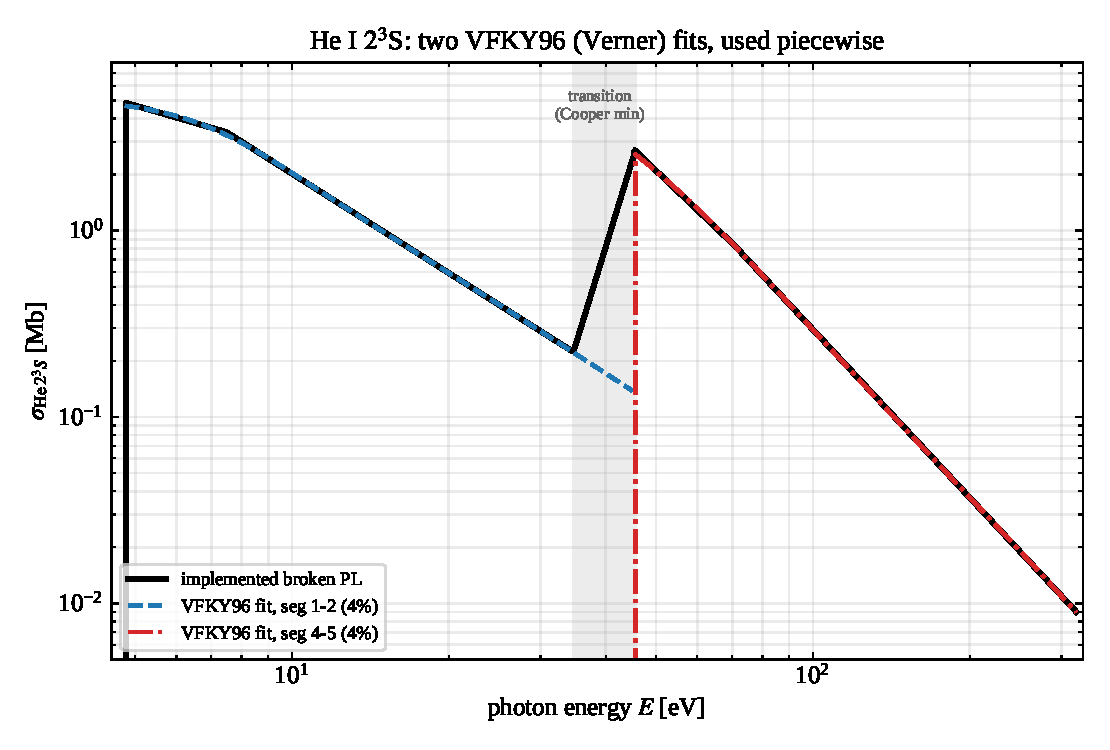
\includegraphics[width=0.74\textwidth]{figures/xsec_HeI23S_vfky.pdf}
\caption{He\,$2^3$S (black: implemented broken power law $+$ TOPbase tail)
with single-VFKY96 fits to segments 1--2 (blue dashed) and 4--5 (red
dash-dot), each good to $\sim$4\%. The shaded band ($34.7$--$45.6\,$eV) is
the Cooper-minimum/rise transition where the two must be spliced piecewise;
a simple sum fails there.}
\label{fig:he23svfky}
\end{figure}

%=============================================================================
\section{Summary}
%=============================================================================

\begin{itemize}
\item EXHALE uses three distinct prescriptions: an exact hydrogenic form
  for H\,I and He\,II, Verner+1996 (VFKY96) for the He\,I ground state
  (default; legacy two-term fit behind \texttt{ATES\_photoionization\_rate}),
  and --- for the He\,I\,$2^3$S triplet --- \textbf{two VFKY96 forms joined
  by a power-law bridge} (\S\ref{sec:he23svfky}; formerly a Norcross-1971
  broken power law, retained commented-out in the code).
\item The He\,I two-term fit agrees with Verner+1996 to within $14\%$
  ($24.6$--$500\,$eV; median $0.94$), running slightly low at
  $50$--$100\,$eV.
\item The He\,I\,$2^3$S broken power law reproduces its parent
  Norcross/p-winds table to within $\sim$$10\%$ ($4.78$--$59\,$eV;
  median $1.00$), including the Cooper minimum and the rise near
  $45\,$eV.
\item An independent check against the \textbf{TOPbase / Opacity Project}
  R-matrix cross section (\S\ref{sec:topbase}) confirms agreement to
  $\sim$$8\%$ in the smooth near-threshold region ($5$--$20\,$eV; median
  $1.00$). TOPbase additionally shows autoionizing resonances above
  $\sim$$35\,$eV (averaged over by the fits) and a smooth tail above
  $59\,$eV (where EXHALE truncates to zero).
\item The $40$--$55\,$eV autoionizing resonances raise the He\,$2^3$S
  rate by only $\sim$$1$--$2\%$ once the few numerically under-resolved
  spikes are excluded (\S\ref{sec:resonance}); the raw TOPbase table must
  not be integrated directly.
\item A simple power law $\sig_{\rm He\,2^3S}\simeq0.294\,(E/100\,\text{eV})^{-2.99}\,\Mb$
  reproduces the resonance-free TOPbase background to $\sim$$5\%$ and
  provides a clean smooth extension above the $59\,$eV cutoff
  (\S\ref{sec:tail}). For a single well-connected cross section over the
  \emph{whole} range, a $15$-node log--log PCHIP table
  (Table~\ref{tab:unified}, \S\ref{sec:unified}) follows the TOPbase
  resonance-averaged background to $\sim$$10\%$ and changes the rate by
  only $+1.7\%$. The \emph{recommended} drop-in (\S\ref{sec:extend})
  keeps the broken power law intact up to the $45.6\,$eV bump and only
  re-aims its last segment (slope $-3.039\!\to\!-2.658$) to meet the
  TOPbase tail $10^{5.462}E^{-2.996}\,\Mb$ at $70\,$eV: continuous at both
  joins, $3\%$ to TOPbase, and $+0.65\%$ in rate.
\item Both fitted helium cross sections are adequate for the
  photoionization balance. Extending the He\,$2^3$S fit above $59\,$eV
  with the TOPbase tail changes its photoionization rate by only
  $0.1$--$1.2\%$ (\S\ref{sec:rateimpact}), so the cutoff is harmless; the
  one worthwhile refinement, if any, is to migrate He\,I to the VFKY96
  form (Table~\ref{tab:vfky}) for internal consistency.
\end{itemize}

%=============================================================================
\section{Reproducing this comparison}\label{sec:script}
%=============================================================================

All figures and numbers are generated by
\texttt{docs/compare\_photoion\_cross\_sections.py}:

\begin{verbatim}
cd ATES/EXHALE/docs
python3 compare_photoion_cross_sections.py
# -> figures/xsec_overview.pdf
#    figures/xsec_HeI_vs_Verner.pdf
#    figures/xsec_HeI23S_vs_pwinds.pdf
#    figures/xsec_HeI23S_topbase.pdf
#    figures/xsec_HeI23S_tail.pdf
#    figures/xsec_HeI23S_unified.pdf
#    figures/xsec_HeI23S_ext.pdf
#    figures/xsec_HeI23S_vfky.pdf
# reads: data/topbase_HeI_2_3S_photo.dat
\end{verbatim}

The TOPbase table was retrieved (once) from the CDS Opacity Project
server with
\begin{verbatim}
curl -L -G "https://cds.unistra.fr/cgi-bin/topbase/topbase.sh" \
  --data "com=dt" --data "ent=p" \
  --data "nz1=2"  --data "nz2=2"  --data "ne1=2" --data "ne2=2" \
  --data "is1=3"  --data "is2=3"  --data "il1=0" --data "il2=0" \
  --data "ip1=0"  --data "ip2=0"  --data "lv1=1" --data "lv2=1" \
  --data "en1=0.0" --data "en2=0.0" --data "so=s1"
\end{verbatim}
and parsed into \texttt{data/topbase\_HeI\_2\_3S\_photo.dat} (photon
energy in Ry $\to$ eV; $\sig$ in Mb).

The script ports \texttt{sigma}, \texttt{sigma\_HeI}, \texttt{sigma\_HeI23S}
and \texttt{sigma\_VFKY96} from \texttt{cross\_sec.f90} (using the same
constants $h_{\rm eV}$, $c$ from \texttt{parameters.f90}), hard-codes the
Verner+1996 He\,I/H\,I/He\,II parameters and the 23-point
p-winds/Norcross table, and emits the three vector-PDF figures.

\end{document}
